%----------------------------------------------------------------------------
\chapter{Helyreállítás tesztelése}
%----------------------------------------------------------------------------

Ebben a fejezetben két jeleneten tesztelem a helyreállítás minőségét. Az elsőben a két kamerát egymás mellé helyezem úgy, hogy képsíkjaik nagyjából egybeessenek, míg a második jelenetnél a két kamera optikai tengelye egy hegyes szöget zár be.

{\color{blue}
A teszteléshez két darab Logitech QuickCam Pro 9000 típusú webkamerát használtam, melyektől VGA felbontású ($640\times 480$) képeket kértem le.
}

% -------------------------------------------------------
\section{Első jelenet}
% -------------------------------------------------------

Elsőként egy olyan jeleneten próbáltam ki az elkészült alkalmazást, amely esetén a két kamera egymás mellett van (lásd \ref{fig:scene1_camerapose}. ábra), egy irányba néznek, és két teás dobozt mozgatok előttük. A jelenet 178 képkockából állt (\textasciitilde 5 másodperc), melyből mindegyik $640\times 480$-as felbontású, színes kép. \Aref{fig:scene1_frames}. ábrán látható a bal oldali kamerák által rögzített 3 képkocka és -- a könnyebb összehasonlíthatóság végett -- ugyanezen nézőpontból vett helyreállításaival együtt. Megfigyelhető, hogy a bal oldali teás doboz rekonstrukciója a textúrázatlan területeken várakozásainknak megfelelően hiányos, hiszen itt nem hagyatkozhattunk az optikai folyam által adódó elmozdulásokra. Ugyanezen okok miatt a szereplő kezeiből is csak néhány pontot lehetett helyreállítani.

\begin{figure}[tbh]
\centering
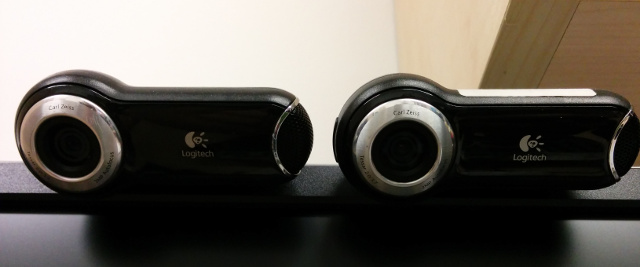
\includegraphics[width=300pt]{figures/scene1_camerapose.jpg}
\caption{Kamerák helyzete az első jelenetnél \label{fig:scene1_camerapose}}
\end{figure}

\begin{figure}[tbh]
\centering
\begin{subfigure}[b]{.32\linewidth}
	\centering
	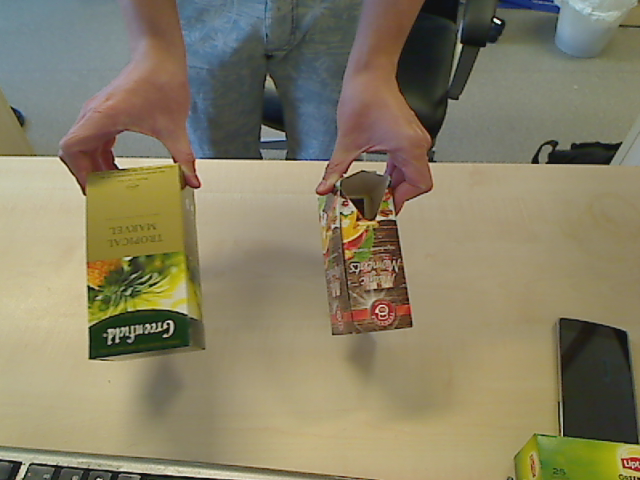
\includegraphics[width=135pt]{figures/left_93.png}
  \end{subfigure}
\begin{subfigure}[b]{.32\linewidth}
	\centering
	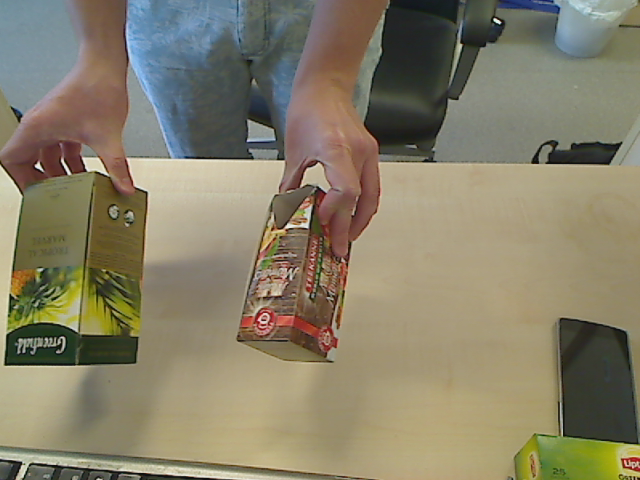
\includegraphics[width=135pt]{figures/left_153.png}
  \end{subfigure}
\begin{subfigure}[b]{.32\linewidth}
	\centering
	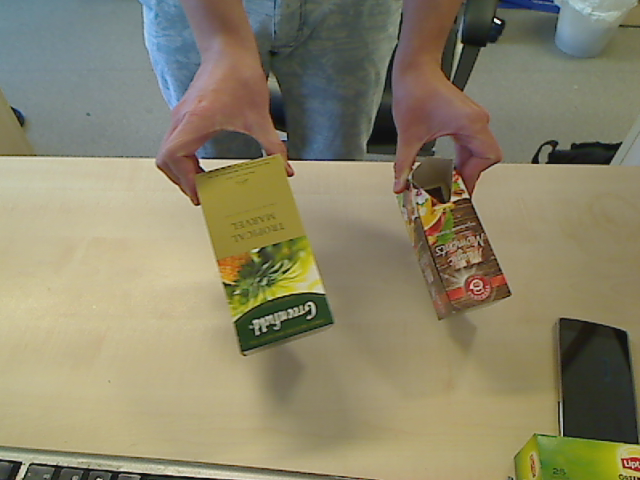
\includegraphics[width=135pt]{figures/left_223.png}
  \end{subfigure}\\\vspace{5pt}
\begin{subfigure}[b]{.32\linewidth}
	\centering
	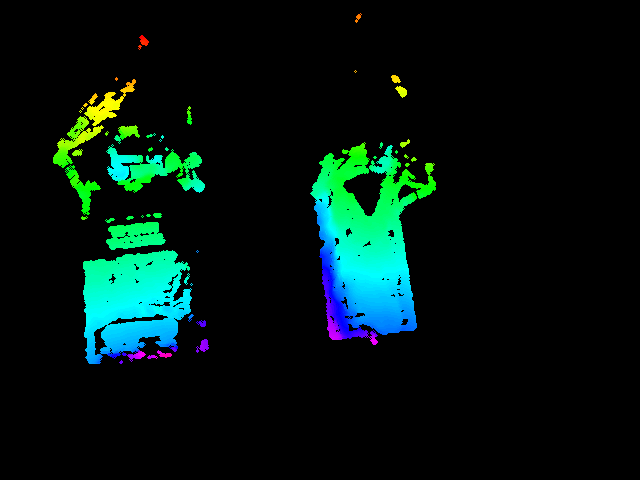
\includegraphics[width=135pt]{figures/vis_93.png}
  \end{subfigure}
\begin{subfigure}[b]{.32\linewidth}
	\centering
	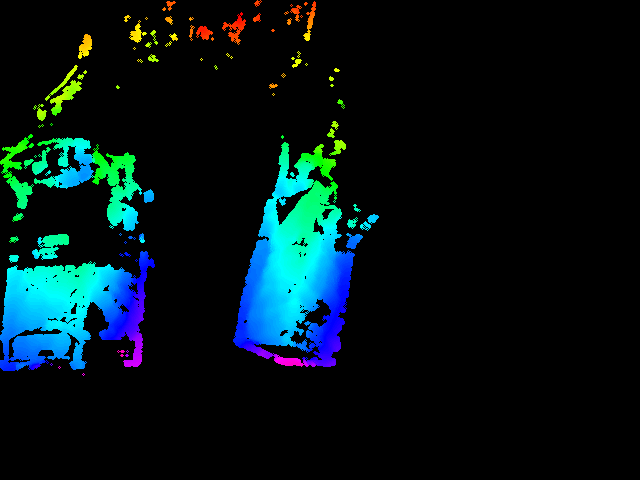
\includegraphics[width=135pt]{figures/vis_153.png}
  \end{subfigure}
\begin{subfigure}[b]{.32\linewidth}
	\centering
	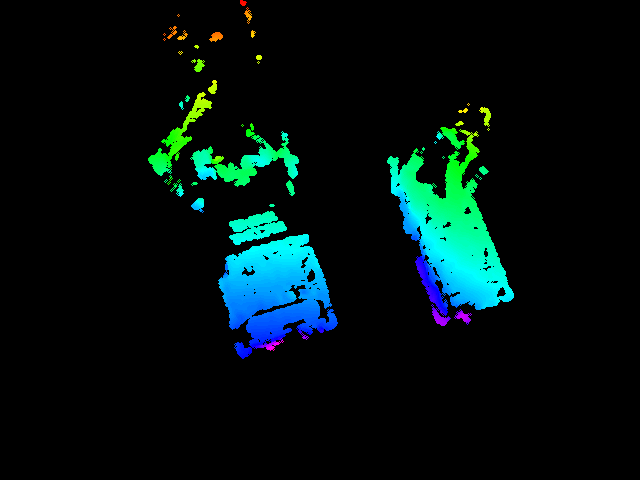
\includegraphics[width=135pt]{figures/vis_223.png}
  \end{subfigure}
\caption{A bal oldali kamera 3 képkockája (40., 100. és 170. képkocka) az első jelenetből, valamint a helyreállított képek a baloldali kamera nézőpontjából \label{fig:scene1_frames}}
\end{figure}

{\color{red} Kicsi értékelés, a képsorból hány volt nagyon jó helyreállítás, mennyi értékelhetetlen, hány képen mennyi objektumot detektáltam. Átlagos sebesség, pixel hiba. Kontúr rajzolás!!!

% -------------------------------------------------------
\section{Második jelenet}
% -------------------------------------------------------

}